\section{Server architecture}
The server is implemented in Dropwizard~\cite{dropwizard}, which is a framework to make RESTful web services. The team chose a RESTful approach because it makes the server easier to interface 
with because it is stateless. The data-interchange format chosen to transfer data between the app and the server is JSON~\cite{json}. This format was chosen for its readability and it is also 
very easily parsed by computer software.

The server exposes a set of endpoints that will have reply when a HTTP request is sent to it. These endpoints provide functionality like syncing of data and fetching friend activity.

The Dropwizard implementation that is used makes it very easy to handle requests and send data 

The data is stored in a MySQL database using the JDBC API and the JDBI abstraction layer.

\begin{figure}[H]
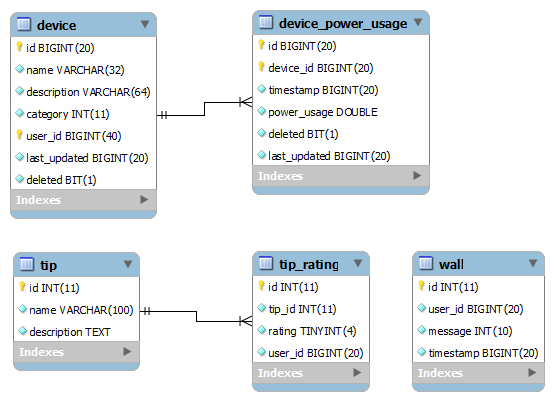
\includegraphics[width=\textwidth]{ch/architecture/fig/ER-Diagram.png}
\caption{ER-Diagram for the database}
\label{fig:ER-Diagram}
\end{figure}